\section{Numerical methods}
\label{sec: numerics}

In this section, different techniques will be presented to solve modal and non-modal stability problems for very large-scale dynamical systems. Such very large-scale systems typically arise from the spatial discretization of partial differential equations, e.g.\ the Navier-Stokes equations in fluid dynamics. Throughout this section, the two-dimensional shear-driven cavity flow at various Reynolds numbers will serve as an example. The same configuration as \cite{??} is considered. The dynamics of the flow are governed by
\begin{equation}
  \begin{aligned}
    \displaystyle \frac{\partial \mathbf{U}}{\partial t} + \left( \mathbf{U} \cdot \nabla \right) \mathbf{U} & = - \nabla P + \frac{1}{Re} \nabla^2 \mathbf{U} \\
    \nabla \cdot \mathbf{U} & = 0,
  \end{aligned}
  \label{eq: numerics -- Navier-Stokes equations}
\end{equation}
where $\mathbf{U}$ is the velocity field and $P$ is the pressure field. Figure \ref{fig: numerics -- shear-driven cavity flow} depicts a typical vorticity snapshot obtained from direct numerical simulation at a supercritical Reynolds number.

Given a fixed point $\mathbf{U}_b$ of the Navier-Stokes equations \eqref{eq: numerics -- Navier-Stokes equations}, the dynamics of an infinitesimal perturbation $\mathbf{u}$ evolving on top of it are governed by
\begin{equation}
  \begin{aligned}
    \displaystyle \frac{\partial \mathbf{u}}{\partial t} + \left( \mathbf{u} \cdot \nabla \right) \mathbf{U}_b  + \left( \mathbf{U}_b \cdot \nabla \right) \mathbf{u} & = - \nabla p + \frac{1}{Re} \nabla^2 \mathbf{u} \\
    \nabla \cdot \mathbf{u} & = 0.
  \end{aligned}
  \label{eq: numerics -- linearized Navier-Stokes equations}
\end{equation}
Once projected onto a divergence-free vector space, Eq. \eqref{eq: numerics -- linearized Navier-Stokes equations} can be formally written as
\begin{equation}
  \dot{\mathbf{u}} = \mathbfcal{A}\mathbf{u},
  \label{eq: numerics -- linearized Navier-Stokes equations bis}
\end{equation}
where $\mathbfcal{A}$ is the linearized Navier-Stokes operator. After being discretized in space, $\mathbfcal{A}$ is a $n \times n$ matrix. For our example, the computational domain is discretized using ??? grid points, resulting in a total of $2 \times ??$ degrees of freedom. From a practical point of view, explicitly assembling the resulting matrix $\mathbfcal{A}$ would require approximately ?? Gb. Investigating the stability properties of this two-dimensional flow would thus not be possible on a simple laptop at the moment despite the simplicity of the case considered. It has to be noted however that, given an initial condition $\mathbf{u}_0$, the analytical solution to Eq. \eqref{eq: numerics -- linearized Navier-Stokes equations bis} reads
\begin{equation}
  \mathbf{u}(T) = \exp \left( \mathbfcal{A}T \right) \mathbf{u}_0,
  \notag
\end{equation}
where $\mathbfcal{M} = \exp \left( \mathbfcal{A}T \right)$ is the exponential propagator introduced previously. Although assembling explicitly this matrix $\mathbfcal{M}$ is even harder than assembling $\mathbfcal{A}$, its application onto the vector $\mathbf{u}_0$ can easily be computed using a classical time-stepping code solving the linearized Navier-Stokes equations \eqref{eq: numerics -- linearized Navier-Stokes equations}. Such a \emph{time-stepper} approach has been popularized by \cite{??}. In the rest of this section, the different algorithms proposed for fixed point computation, linear stability and non-modal stability analyses will heavily rely on this time-stepper strategy. The key point is that they require only minor modifications of an existing time-stepping code to be put into use.

  %%%%%%%%%%%%%%%%%%%%%%%%%%%%%%%%%%%%%%%%%%%%%%%%%%%%%%%
  %%%%%                                             %%%%%
  %%%%%     KRYLOV METHODS FOR LINEAR EQUATIONS     %%%%%
  %%%%%                                             %%%%%
  %%%%%%%%%%%%%%%%%%%%%%%%%%%%%%%%%%%%%%%%%%%%%%%%%%%%%%%

  % \subsection{Krylov methods for for solving linear systems}
  % \label{subsubsec: theory -- krylov methods}



  %%%%%%%%%%%%%%%%%%%%%%%%%%%%%%%%
  %%%%%                      %%%%%
  %%%%%     FIXED POINTS     %%%%%
  %%%%%                      %%%%%
  %%%%%%%%%%%%%%%%%%%%%%%%%%%%%%%%

  \subsection{Fixed points computation}
  \label{subsec: numerics-fixed points computation}

  The starting point when investigating a nonlinear dynamical system it to determine its fixed points. As discussed in \textsection \ref{subsec: theory-fixed points}, for a continuous-time dynamical system, such points are solution to
  \begin{equation}
    \mathbfcal{F} \left( \mathbf{X} \right) = 0,
    \label{eq: numerics -- continuous-time fixed point}
  \end{equation}
  while one needs to solve
  \begin{equation}
    \mathbf{X} - \mathbfcal{G} \left( \mathbf{X} \right) = 0
    \label{eq: numerics -- discrete-time fixed point}
  \end{equation}
  for a discrete-time nonlinear dynamical system. In this section, three different fixed point solvers will be presented.

    %-----> Selective frequency damping.
    \subsubsection{Selective Frequency Damping}

    Selective frequency damping is a fixed point computation technique proposed by {\AA}kervik \emph{et al.}\ \cite{pof:akervik:2006} in 2006 and largely adapted from the original work of Pruett \emph{et al.}\ \cite{pof:pruett:2003, pof:pruett:2006} on temporal approximate deconvolution models for large-eddy simulations. It has since become one of the standard approaches for fixed point computation in fluid dynamics due to its ease of implementation. Note that various implementations of the original selective frequency damping method have been proposed over the years \cite{pof:jordi:2014, pof:jordi:2015, pof:cunha:2015}. Moreover, it has since been extented to compute steady states of the Reynolds-Averaged-Navier-Stokes (RANS) equations \cite{cf:richez:2016} as well as for the computation of unstable periodic orbits \cite{prf:leopold:2017}. In the rest of this section, only the original formulation by {\AA}kervik \emph{et al.}\ \cite{pof:akervik:2006} will be described.

    Let us consider a fixed point $\mathbf{X}^*$ of the nonlinear system
    $$\dot{\mathbf{X}} = \mathbfcal{F} \left( \mathbf{X} \right).$$
    If $\mathbf{X}^*$ is linearly unstable, then any initial condition $\mathbf{X}_0 \neq \mathbf{X}^*$ will quickly depart from $\mathbf{X}^*$. Using standard regularization techniques from control theory, the aim of selective frequency damping is thus to stabilize the linearly unstable fixed point $\mathbf{X}^*$. For that purpose, one can use proportional feedback control so that the forced system now reads
    \begin{equation}
      \dot{\mathbf{X}} = \mathbfcal{F} \left( \mathbf{X} \right) - \chi \left( \mathbf{X} - \mathbf{Y} \right),
      \label{eq: numerics -- sfd forced system}
    \end{equation}
    where $\chi$ is the control gain and $\mathbf{Y}$ the target solution. This target solution is obviously the fixed point one aims to stabilize, i.e.\ $\mathbf{Y} = \mathbf{X}^*$, which is unfortunately not known \emph{a priori}. It has to be noted however that, for a large range of situations, the instability of the fixed point $\mathbf{X}^*$ will tend to give rise to unsteady dynamics. In such cases, the target solution $\mathbf{Y}$ is thus a modification of $\mathbf{X}$ with \emph{reduced temporal fluctuations}, i.e.\ a temporally low-pass filtered solution. This filtered solution is defined as
    \begin{equation}
      \mathbf{Y}(t) = \mathcal{H}(t, \Delta) * \mathbf{X}(t-\tau)
      \label{eq: numerics -- low-pass filtered solution}
    \end{equation}
    where $\mathcal{H}$ is the convolution kernel of the applied causal low-pass filter and $\Delta$ the filter witdh. Using such definitions, the forced system \eqref{eq: numerics -- sfd forced system} can thus be rewritten as
    \begin{equation}
      \dot{\mathbf{X}} = \mathbfcal{F}\left( \mathbf{X} \right) - \chi \left( \mathbfcal{I} - \mathcal{H} \right) * \mathbf{X}.
      \label{eq: numerics -- sfd foced system bis}
    \end{equation}
    As $\mathbf{X}$ tends to the fixed point $\mathbf{X}^*$, the low-pass filtered solution $\mathbf{Y}$ tends to $\mathbf{X}$. Once a steady state has been reached, one has
    $$\mathbf{X} = \mathbf{Y} = \mathbf{X}^*,$$
    i.e.\ the fixed point of the controlled system \eqref{eq: numerics -- sfd foced system bis} is the same as that of our original system. Moreover, as the system approaches its fixed point, the amplitude of the proportional feedback control term vanishes.

    \paragraph{Applying the low-pass filter in the time domain}

    As it is formulated, computing the low-pass filtered solution \eqref{eq: numerics -- low-pass filtered solution} requires the evaluation of the following convolution integral
    \begin{equation}
      \mathbf{Y}(t) = \int_{-\infty}^t \mathcal{H}(\tau-t, \Delta) \mathbf{X}(\tau) \mathrm{d}\tau.
      \label{eq: numerics -- convolution integral}
    \end{equation}
    Note that, to be admissible, the kernel $\mathcal{H}$ must be positive and properly normalized. Moreover, in the limit of vanishing filter width, it must approach the Dirac delta function. To the best of our knowledge, all implementations of the selective frequency damping thus relies on the exponential kernel
    \begin{equation}
      \mathcal{H}(\tau - t, \Delta) = \displaystyle \frac{1}{\Delta} \exp \left( \frac{\tau - t}{\Delta} \right).
      \label{eq: numerics -- exponential kernel}
    \end{equation}
    The corresponding Laplace transform is given by
    \begin{equation}
      \hat{\mathcal{H}}(\omega, \Delta) = \displaystyle \frac{1}{1 + i \omega \Delta}.
      \label{eq: numerics -- laplace transform}
    \end{equation}
    The cutoff frequency of this filter is given by $\omega_c = \nicefrac{1}{\Delta}$. Figure \ref{fig: numerics -- lapalce transform} depicts the real part of $\hat{\mathcal{H}}$ as a function of the frequency $\omega$ for $\Delta=1$. Naturally, this cutoff frequency needs to be tuned so that the frequency associated to the instability one aims to kill is quenched by the filter.

    For real applications, evaluating the convolution integral \eqref{eq: numerics -- convolution integral} is impractical as it necessitates the storage of the complete time history of $\mathbf{X}$. Consequently, it is replaced by its differential form given by
    \begin{equation}
      \dot{\mathbf{Y}} = \displaystyle \frac{1}{\Delta} \left( \mathbf{X} - \mathbf{Y} \right)
      \label{eq: numerics -- differential filter formulation}
    \end{equation}
    which can be integrated in time using classical integration schemes, e.g.\ second-order backward Euler. Combining \eqref{eq: numerics -- differential filter formulation} and \eqref{eq: numerics -- sfd forced system} finally yields to the following extended system
    \begin{equation}
      \left\{
      \begin{aligned}
        \dot{\mathbf{X}} & = \mathbfcal{F}\left( \mathbf{X} \right) - \chi \left( \mathbf{X} - \mathbf{Y} \right) \\
        \dot{\mathbf{Y}} & = \displaystyle \frac{1}{\Delta} \left( \mathbf{X} - \mathbf{Y} \right).
      \end{aligned}
      \right.
      \label{eq: numerics -- selective frequency damping}
    \end{equation}
    Implementing \eqref{eq: numerics -- selective frequency damping} into an existing time-stepping code requires only minor modifications, hence making it an easy choice for fixed point computation. It must be emphasized however that, because it relies on a low-pass filtering procedure, this selective frequency damping method is unable to quench non-oscillating instabilities, e.g.\ instabilities arising due to a pitchfork bifurcation. This particular point is one of its major limitations.

    \begin{figure}[b]
      \sidecaption
      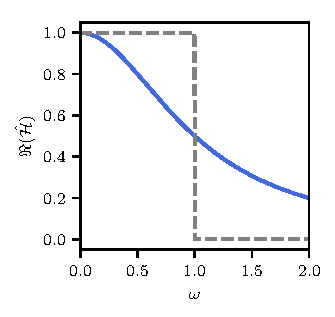
\includegraphics[scale=1]{S3_SFD_transfer_function}
      \caption{Evolution of $\Re \left( \hat{\mathcal{H}} \right)$ ({\color{blue} ---}), i.e.\ the real part of the Laplace transform of the exponential filter, as a function of the frequency $\omega$ for $\Delta=1$. The gray dashed line depicts the ideal spectral cutoff filter.}
      \label{fig: numerics -- lapalce transform}
    \end{figure}

    %-----> Newton-Krylov method.
    \subsubsection{Newton-Krylov method}

    %-----> BoostConv.
    \subsubsection{BoostConv}


    %-----> Comparison.
    \subsubsection{Comparison of the different approaches}


  %%%%%%%%%%%%%%%%%%%%%%%%%%%%%%%%%%%%%%%%%%%%
  %%%%%                                  %%%%%
  %%%%%     MODAL STABILITY ANALYSIS     %%%%%
  %%%%%                                  %%%%%
  %%%%%%%%%%%%%%%%%%%%%%%%%%%%%%%%%%%%%%%%%%%%

  \subsection{Linear stability and eigenvalue computation}

    %-----> Power Iteration.
    \subsubsection{Power Iteration method}

    %-----> Arnoldi decomposition.
    \subsubsection{Arnoldi decomposition}

    %-----> Krylov-Schur decomposition.
    \subsubsection{Krylov-Schur decomposition}




  %%%%%%%%%%%%%%%%%%%%%%%%%%%%%%%%%%%%%%%%%%%%%%%%
  %%%%%                                      %%%%%
  %%%%%     NON-MODAL STABILITY ANALYSIS     %%%%%
  %%%%%                                      %%%%%
  %%%%%%%%%%%%%%%%%%%%%%%%%%%%%%%%%%%%%%%%%%%%%%%%

  \subsection{Non-modal stability and singular value decomposition}

    %-----> Optimal perturbation.
    \subsubsection{Optimal perturbation analysis}

    %-----> Resolvent analysis.
    \subsubsection{Resolvent analysis}
